\subsection{Results}\label{sec:m4:results}
    ~\cref{fig:m4:angular_power_spectrum} shows the angular power spectrum as function of photon multipole $l$. The blue drawn line is the main power spectrum, while the dotted lines are the four constituents of the power spectrum that arise from the source function in ~\cref{eq:m3:theory:source_function}. The red lines are observations taken from ~\cite{Planck2020}, and the turquoise shade shows the theoretical cosmic variance as given in ~\cref{eq:m4:theory:cosmic_variance}. As expected, since we ignore both polarisation and neutrinos there is a discrepancy between the observed values and the theoretical prediction. This is most prominent for larger $l$-s where the observational constraints are low due to high statistical accuracy. In discussing this results, we will focus on the three main parts of the plots, namely the \textit{Sachs-Wolfe plateau} for low $l$-s, the \textit{acoustic oscillations} for intermediate $l$-s and the \textit{diffusion damping} for high $l$-s. Lastly we discuss the matter power spectrum in, where we have obtained the observational data from ~\cite{Chabanier_2019} and ~\cite{Hlozek_2012}.
    \begin{figure}
        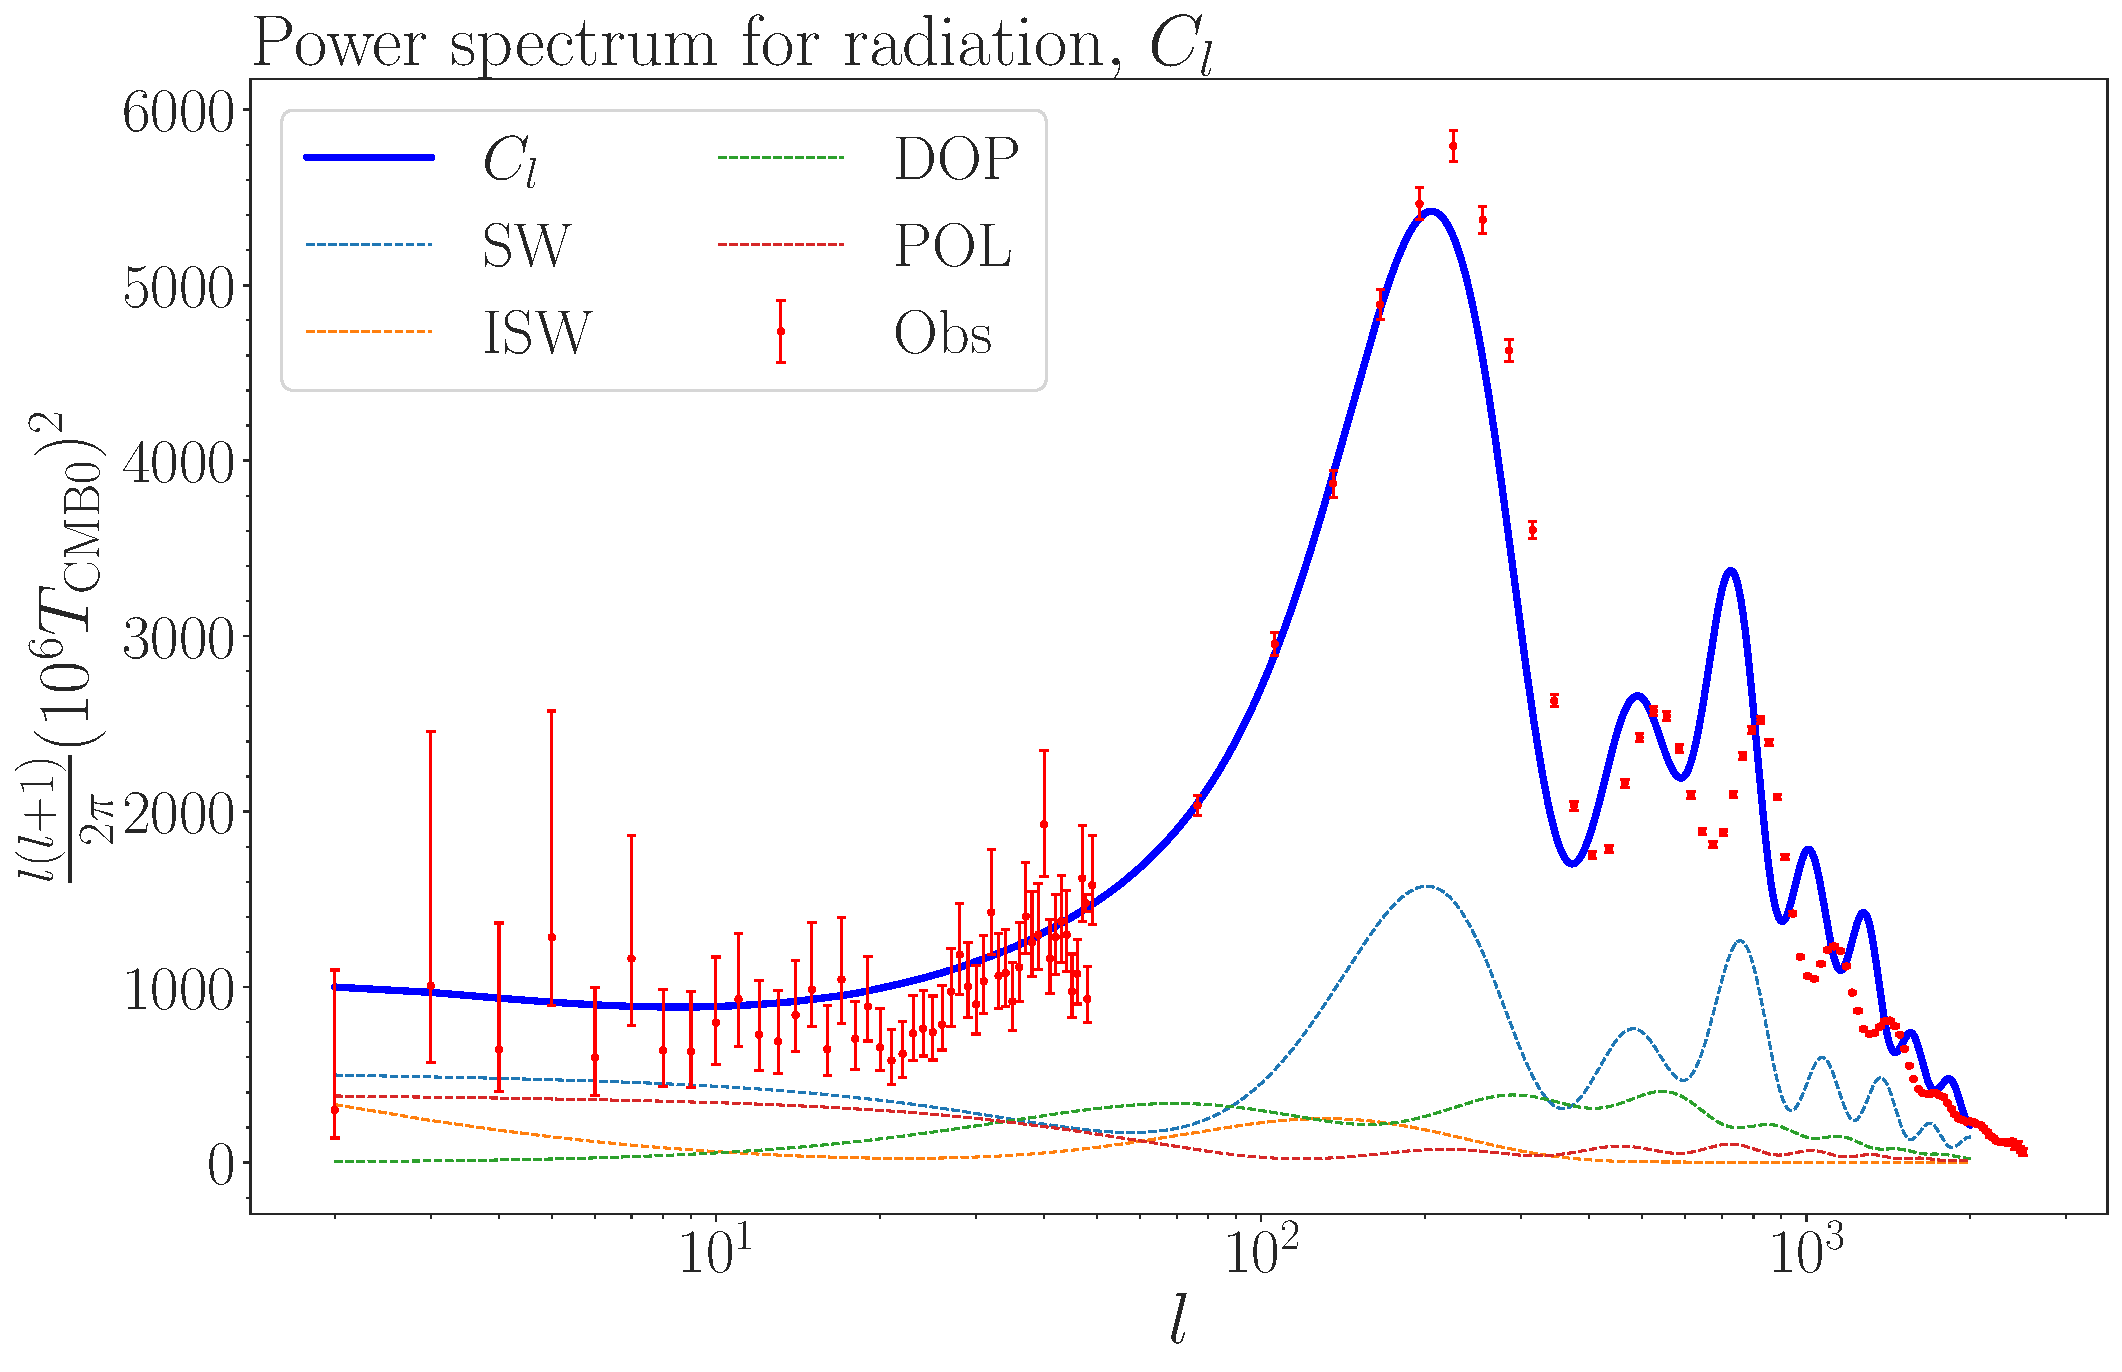
\includegraphics[width=\linewidth]{power_spectrum.pdf}
        \caption{Angular power spectrum as function of photon multipole $l$. The blue line shows the angular power spectrum itself with the intrinsic cosmic variance overplotted in turquoise. The dotted lines are the individual effect of the different constituents of the source function. The red error bars are observational constraints.}
        \label{fig:m4:angular_power_spectrum}
    \end{figure}
    \subsubsection{The Sachs-Wolfe plateau}
        The Sachs-Wolfe plateau is the part of the angular power spectrum that appear fairly flat for low $l$, i.e. large scales, hence it names. These large scale represent modes that had not yet entered the horison at the time of recombination. According to the Sachs-Wolfe (SW) term in the source function in ~\cref{eq:m3:theory:source_function}, the major contribution to the power spectrum are the temperature anisotropies present at the last scattering surface. This is the main contributor to the transfer function and thus the power spectrum itself. These effects are described by the photon monopole, and the value of the gravitational perturbation, $\Psi$, whose main effect slowed the photons down through gravitational redshift.\footnote{Plus a small quadrupole correction.} For large scales, that have not yet entered the horison at the time of last scattering, the fluctuation to the gravitational perturbation have not yet been affected by causal physics. As a result, they closely resemble the initial perturbations induced by inflation. 

        Thus, the Sachs-Wolfe plateau may be understood as a tracer of the primordial power spectrum. If we continue to assume this take the form of a Harrison-Zel'dovich spectrum parametrised by the amplitdue $A_s$ and spectral index $n_s$ we are able to estimate the former by considering the amplitude of the Sachs-Wolfe plateau, and the latter by its shape. $n_s=1$ would generate a flat primordial power spectrum, whereas $n_s>1$ would give emphasis to small scales and vice versa. 

        We also take note of the large cosmic variance in this region. As already explained, this is and intrinsic feature of the angular power spectrum when comparing to observations, as we only have one universe to make observations in. The observational constraints are also significantly less accurate in this region, which is to be expected. 
        
        In figure ~\cref{fig:m4:angular_power_spectrum} we also see some contribution from the integrated Sachs-Wolfe (ISW) term, which occur due to changes in the gravitational potentials. Most prominent in the discussion of the Sachs-Wolfe plateau is the late-time ISW which occur around matter-dark-energy equality. These effects can be seen for the largest scales, as they happened quite recently, and contributes to the minor deviations away from a straight line for the Sachs-Wolfe plateau.
        
        There is also an increasing contribution of the Doppler term, which correspond to the peculiar velocity of matter (and our peculiar velocity relative to the CMB-frame). The Sachs-Wolfe plateau indicate the existence of large scale structures in the Universe, because of its power at the smallest $l$-s. It also provides valuable insight into the primordial power spectrum, and the process of inflation. 

    \subsubsection{Acoustic oscillations}
        The acoustic oscillations seen at intermediate scales in ~\cref{fig:m4:angular_power_spectrum} are a result of oscillations in the primordial plasma\footnote{Plasma containing tightly coupled baryons and photons, giving rise to the alternative name; \textit{baryon acoustic oscillations (BAO)}.} in the very early universe. These oscillations are a result of primordial fluctuations in the dark matter distribution, effectively creating gravitational wells in which baryonic matter accumulate. In areas where the density of baryonic matter is increased, so is the photon pressure as well, due to their tight coupling. The gravitational wells thus have an attractive effect on the primordial plasma while the photon pressure have a repulsive effect. The interplay between these two effect source acoustic oscillations that travel throughout the universe. 

        The physics of gravitational attraction and radiative repulsion are both causal, so the effects from these phenomena may only be conveyed within causally connected regions. Thus, the scale for which these oscillations may be observed is closely governed by the causal horison. Another thing to keep in mind is that this interplay between gravitational attraction and radiative repulsion require photons to be coupled to baryons. Therefore, we would think that the acoustic oscillations present at the last scattering surface is imprinted on the CMB and thus the angular power spectrum.

        The first peak at around $l\sim200$ represent the first contraction of the plasma. In order to have repulsion, there must first be attraction, thus this must have happened first. This contraction and subsequent rarefaction creates these oscillations in the primordial plasma, propagating with the speed of sound (found in ~\cref{eq:m2:theory:sound_speed}). The quantity measured in the angular power spectrum is the temperature fluctuations, not the oscillations themselves. However, the Sachs-Wolfe effect tells us that the radiation escaping from these oscillating fluctuations looses energy due to gravitational redshift. Anomalies in photon temperature are thus tracers of the potential wells from which these oscillations occur. Since most photons we observe today have free-streamed to us from the surface of last scattering, the peaks and troughs of the angular power spectrum represents the different scales affected by these propagating oscillations at the time of last scattering. The first peak represents the largest of these scale, i.e. the scale corresponding to the sound horison at the time of last scattering. In other word, it is the variation in photon temperature due to the very first contraction of the primordial fluid. 

        The second and third peak subsequently correspond to the first rarefaction and the second compression. These temperature fluctuations occur at smaller scales because they happened at a later time, leaving less time for the sound waves to propagate, resulting in a smaller angular scale at the time of recombination. In fact, it is fair to assume that the imprint of each scale happens at slightly different times, since the \textit{freeze-in} ultimately occur when the mean free path of photons becomes larger than the scale of the oscillating wave. However, in cosmic time these events are very close to each other, as the mean free path increased rapidly during recombination. Similar arguments follow for the next peaks, but these are greatly affected by damping. It is also worth noting that the acoustic oscillations seen in ~\cref{fig:m4:angular_power_spectrum} are mostly a result of the Sachs-Wolfe effect, i.e. the fluctuations of the gravitational potential at the time of last scattering. There is also a small contribution from the doppler term. \TODO{why?} 

    \subsubsection{The damping tail}
        In the primordial plasma that existed before recombination, photons were tightly coupled to baryons (matter) via Thomson scattering. This resulted in an opaque environment, where photons had a short mean free path, and energy was interchanged with every collision. These interactions and consequent energy transfers caused the temperature fluctuations at small scales to be smoothed. In terms of angles, it is fair to assume that the scattering of photons off electrons causes a dispersion across all angles, as none should be favoured. All of this results in an averaging of the temperature in local neighborhoods, effectively reducing the temperature fluctuations. The smaller the scale, the greater the effect. This phenomenon is called \textit{silk damping} or more generally \textit{diffusion damping}, ~\cite{dodelson2020modern}. In ~\cref{fig:m4:angular_power_spectrum} this can be observed as a damping tail towards the higher $l$-s, where the amplitude of the temperature fluctuations rapidly decrease, but still oscillating. The effect of the diffusion damping is thus to suppress the acoustic oscillations. 

    \subsubsection{Parameter dependence}
        So far we have studied how the angular power spectrum actually appear with our choice of parameters, but how would this appearance change if we changed any of the free parameters? Let's start with the curvature parameter $\O_{k0}$: In our fiducial cosmology, the universe is almost completely flat. If however, we had an open universe ($\O_{k0}>0$), the entire power spectrum would have been shifted towards the right, i.e. towards smaller scales. There are two ways of seeing this; firstly, for an open universe to exist, the acceleration of the expansion need to be large, in order to counteract and eventually rip apart the gravitational force. This faster expansion cools the universe down quicker, and thus recombination happens at an earlier time. Thus, the sound horison at this time must be smaller, and the fluctuations of the photons leaving it must also be present at a smaller scale. This corresponds to the first peak being present at larger $l$. From a geometrical point of view, an open universe is characterised by a hyperbolic conformal distance. This means that an angular separation measured today appears smaller than it actually is, emphasising the shift towards smaller scales for an open universe. Exactly the opposite argument may be used in order to explain why a closed universe would shift the spectrum towards larger scales. Similar effects would be seen if we changed the dark energy component, as this amounts to changing the acceleration of the expansion. 

        Let's consider dark matter next. The primordial gravitational perturbation that give rise to the acoustic oscillations are a result of all matter involved. Dark matter does not couple to photons, and thus increasing the dark matter in the universe would amount to just deepen the primordial potential wells, making the change in gravitational potential the photons need to climb through larger. This enhanced gravitational redshift causes larger fluctuations in the photon temperature resulting in more power in the angular power spectrum, across all scales subjected to acoustic oscillations. Thus, increasing the cold dark matter would increase the power of the acoustic oscillations and vice verse. 

        In term of baryonic matter, increasing it would make the compressions more powerful by accreting more matter per compression and deepen the well, which in turn force the photons emitted to climb out from a deeper potential. The radiative pressure will govern the rarefaction, and thus the gravitational blueshift of the photons. Thus, increasing radiation as well would increase the power of the rarefaction. Therefore, increasing baryonic matter would give more power to the odd peaks of the spectrum, whereas icreasing radiation would give more power to the even peaks. Thus, the ratio between baryonic matter and radiation modulates the height of peaks, ~\cite{Hu_1996}.

    \subsubsection{The matter power spectrum}
    
    \begin{figure}
        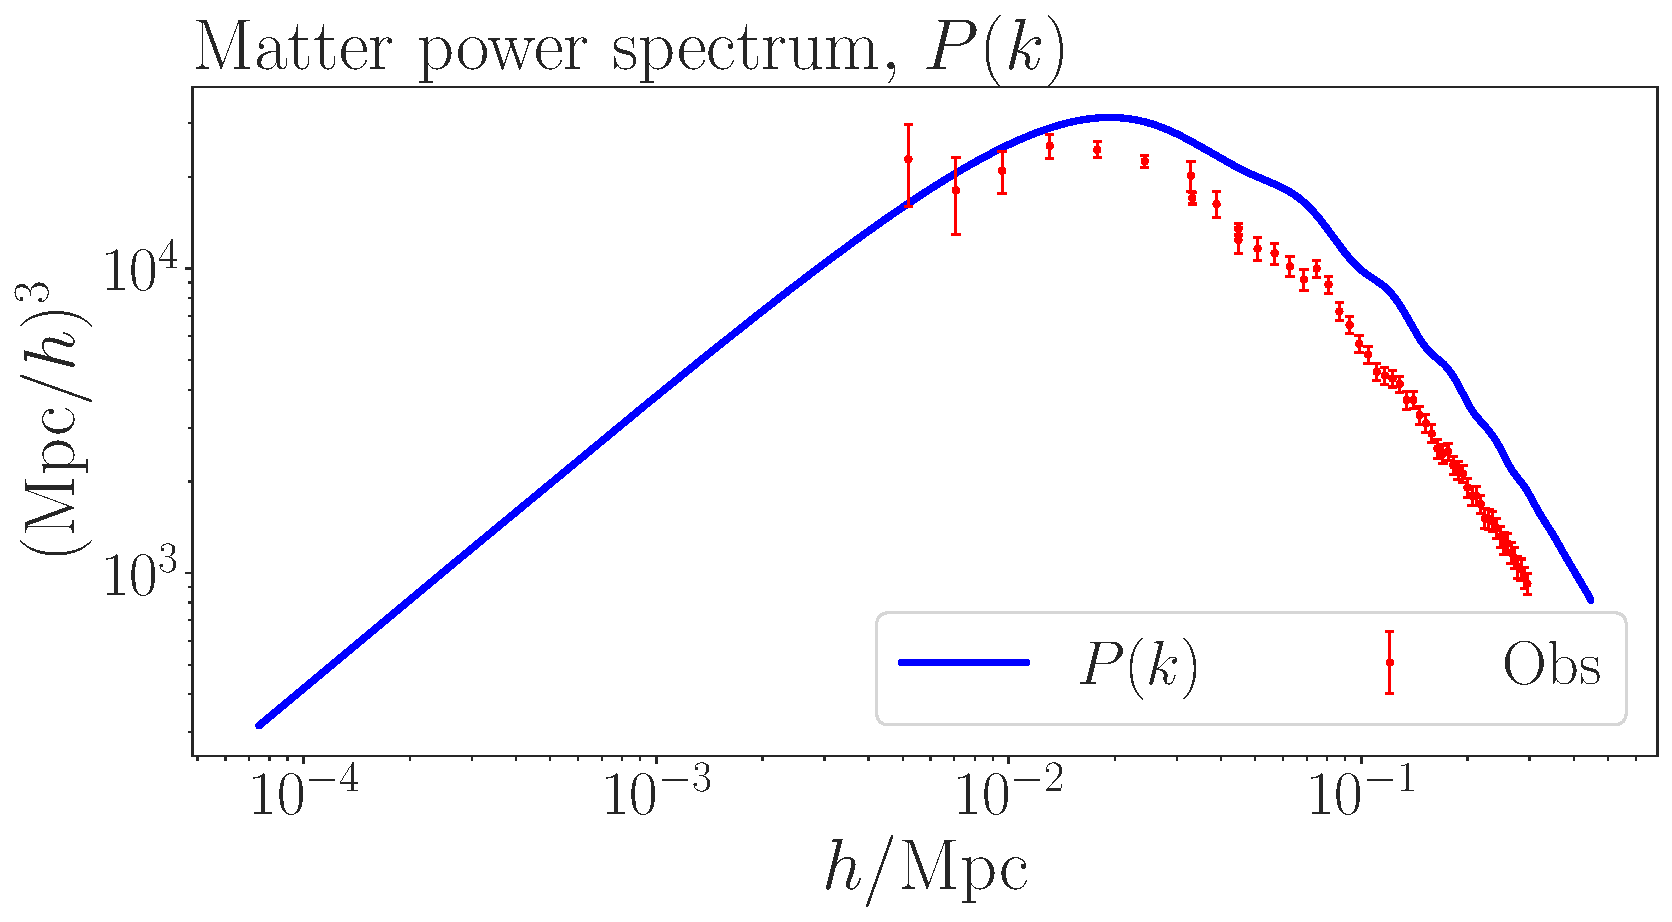
\includegraphics[width=\linewidth]{matter_power_spectrum.pdf}
        \caption{Matter power spectrum as function of wavenumber $k$. The violet dotted line the equality scale, which is the wavenumber that correspond to the mode entering the horison at the time of radiation-matter equality. The red error bars are observational constraints.}
        \label{fig:m4:matter_power_spectrum}
    \end{figure}